\documentclass{svproc}

% to typeset URLs, URIs, and DOIs
\usepackage{url}
\def\UrlFont{\rmfamily}

% The following packages can be found on http:\\www.ctan.org
\usepackage{graphics} % for pdf, bitmapped graphics files
\usepackage{epsfig} % for postscript graphics files
\usepackage{mathptmx} % assumes new font selection scheme installed
\usepackage{times} % assumes new font selection scheme installed
\usepackage{amsmath} % assumes amsmath package installed
\usepackage{amssymb}  % assumes amsmath package installed
\usepackage{caption}
\usepackage{subcaption}
\usepackage{array}
\usepackage{siunitx}
\usepackage{tabularx}
\usepackage[T1]{fontenc}
\usepackage{makecell}
\usepackage{biblatex}
\bibliography{bibliography}

\begin{document}
\mainmatter              % start of a contribution
\title{
Laser tracker placement optimization for highly flexible manufacturing systems
}
\titlerunning{Laser tracker placement}


% latex magic to format multiple authors affiliations
\newcommand*\samethanks[1][\value{footnote}]{\footnotemark[#1]}
\makeatletter
% *, 2, 3, ...
\renewcommand*{\@fnsymbol}[1]{\ifcase#1\or\@arabic{#1}\else*\fi}
\makeatother

\author{Jan Baumgärtner \inst{1,2},
Max Goebels \inst{1,2,3},   Alexander Puchta \inst{1,2} and Jürgen Fleischer\inst{1}% <-this % stops a space
}
\institute{wbk Institute of Production Science, Karlsruhe Institute of Technology,
76131 Karlsruhe, Germany 
\and
These authors contributed equally to this work.
\and
Corresponding: \email{max.goebels@kit.edu}
}%

\authorrunning{Baumgärtner et al.}%
\tocauthor{Jan Baumgärtner, Max Goebels, Alexander Puchta, and Jürgen Fleischer}%

\maketitle

\begin{abstract}
In recent years, modular and reconfigurable manufacturing systems have gained attention for their fast adaptability towards product changes.
While system design is now highly automated, designing the verification setup remains a manual design problem involving tasks like placing external sensors to measure performance.
This paper argues that design optimization approaches for manufacturing systems can also automate the design of the verification setup.
This is demonstrated by placing a laser tracker system with markers, which can be challenging to design due to their line-of-sight complexity and simultaneous measurement of multiple systems.
We present a straightforward optimization approach to demonstrate potential automation in this area.
\keywords{flexible manufacturing systems, sensor placement optimization, laser tracker, particle swarm optimization}
\end{abstract}
\section{Introduction}
The global market for flexible manufacturing systems (FMS) is experiencing significant growth, driven by the increasing demand for customized products and shorter product life cycles~\cite{westkaemperEinfuehrungOrganisationProduktion2006}. FMS are characterized by their ability to adapt to changing requirements, such as variations in product design, production volume, and production sequence. Modular reconfigurable machine tools (MRMT) are a key component of FMS, as they can modify their physical structure to meet evolving product requirements~\cite{Padayachee2012}.
The majority of research in the field of MRMT has concentrated on the development of architectures that adhere to open or semi-open standards, the modular components, and methods for optimizing configurations based on performance metrics~\cite{gadallaRecentAdvancesResearch2017, xuMethodDesignModular2017}.
Despite the aforementioned advancements, a significant gap in the research field remains: the verification of the performance of the aforementioned proposed configurations is often limited to simulations, which are susceptible to a reality gap. Alternatively, manual experimental setups using external sensors are used. However, these manual setups are not only time-consuming but also require expert knowledge.
To address this issue, our paper introduces an automated approach to task-based sensor placement optimization for the verification of MRMT. For the purposes of this study, we consider a robot cell to be an ideal test case for the proposed approach, providing an upper bound for the complexity of task trajectories. This is based on the recognition that although the reconfiguration of robot cells is less pronounced, the task trajectories within them are typically more complex than those typically found in MRMT applications.
\section{State of the art}
The work presented in this paper intersects two research fields: manufacturing systems optimization and sensor placement optimization.
Our primary question is what aspects of a manufacturing system we need to verify.
We focus on system-based verification rather than product-based, aiming to measure the performance of the manufacturing system, not the resulting product quality.
In particular we focuss on approaches that solves what~\cite{reconfigurable_production} calls reconfiguration design problem.
This involves either combining fixed modules to form a system or directly optimizing the systems physical design.
Examples include robot cell optimization problems~\cite{previous_work, stiffness_placement} and robot design optimization problems~\cite{task_synthesis, ad-hoc_manipulator, multi_objective}.
For a manufacturing perspective, works such as~\cite{johannes_1, johannes_2} are relevant.
All of these approaches focus on phyiscal capabilities such as payload, accuracy, stiffness, force, weight, and motion.
To verify that the optimized system configuration achieves the desired performance, we need to measure the system's performance using external sensors,
however in all of the above works the sensor placement for verification (if done at all) is done manually.
This can be a challening task which brings us to the field of sensor placement optimization.
The goal here is to find the optimal sensor placement for accurate system performance measurement.
A adjacent engineering discipline in which sensor placement optimization is a already well studied is structural health monitoring~\cite{shms}.
Here key algorithms where already identified such as genetic algorithms, particle swarm optimization, and simulated annealing~\cite{shms}.
Based on these works we will also use a particle swarm optimization algorithm for our problem.
However the field of structural health monitoring mainly considers static systems while our manufacturing systems are by nature dynamic.
This introduces additional challenges since the sensor placement needs to account for the systems total trajectory.
This challenge has only recently been addressed in manufacturing systems~\cite{ieee_sensors}. Although this early work focuses on process control, not system verification, its methodologies are applicable,
emphasizing optimizing an objective integrated over total process time.
However, since we are not using cameras as in the previous study, we must derive our own visibility model reflecting the measurement characteristics of a laser tracker.
This will be the focus of the next section.

\section{Formulation of the optimization problem}
To solve the joint optimization problem of marker and laser tracker pose, we first need to define the objective function.
Our goal is to maximize the visibility of the marker to the laser tracker.
Similar to approaches such as~\cite{ieee_sensors} we divide the visibility into two components.
Line of sight visibility and field of view visibility.
Both  are depicted in figure~\ref{fig:visibility}.
\begin{figure}
        \centering
        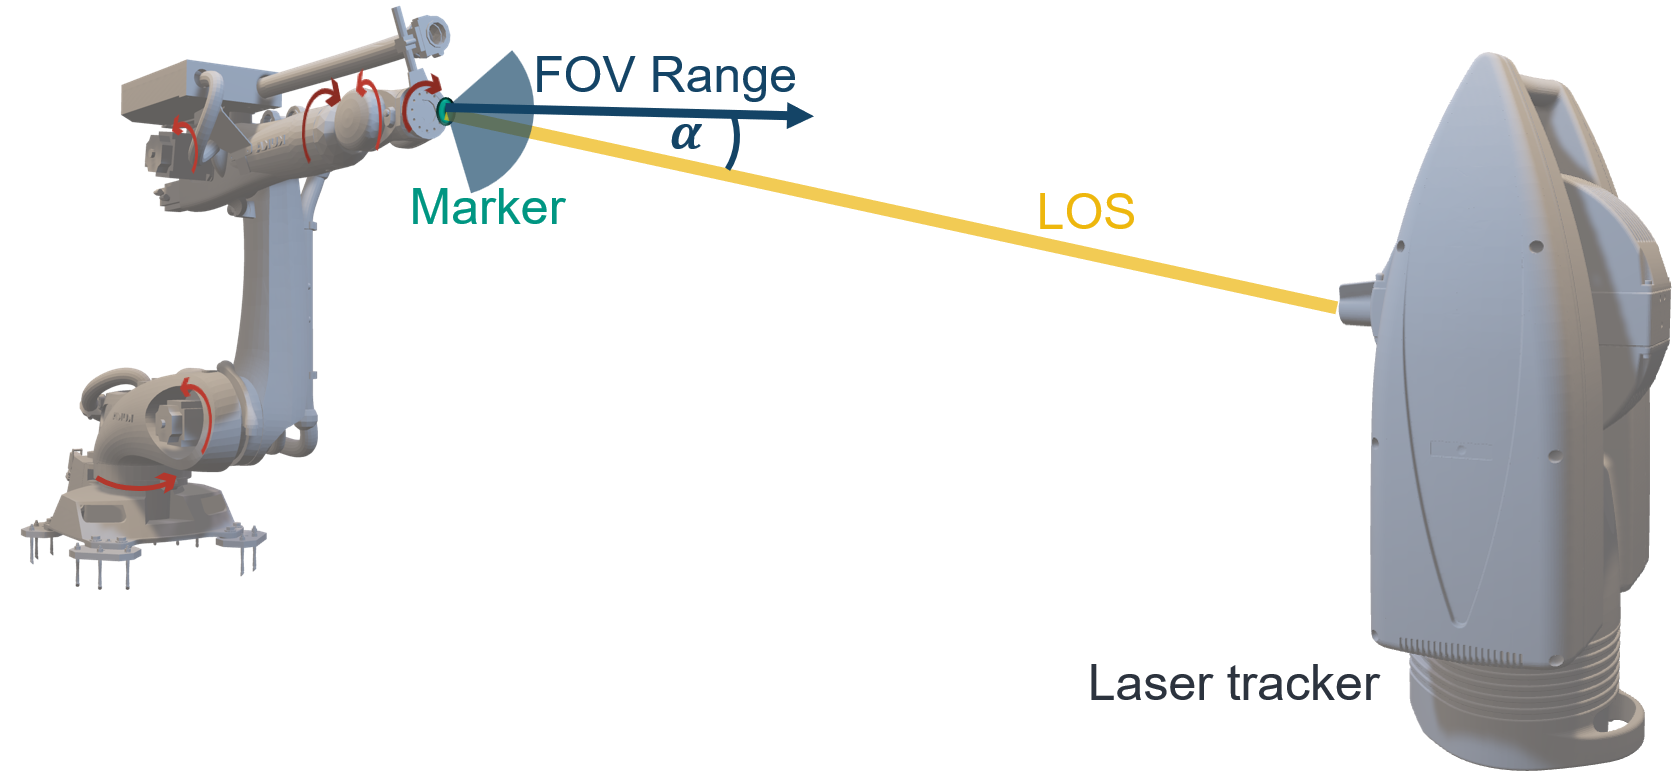
\includegraphics[width=0.7\textwidth]{figures/visibility.png}
        \caption{Field of view (FOV) angle range and line of sight (LOS) components of marker visibility}
        \label{fig:visibility}
\end{figure}
Mathematically we can define line of sight visibility (los visibility) as the following binary function:
\begin{equation}
    f(p_m,p_l) = \begin{cases}
    -1 & \text{if } \text{marker is in line of sight of the laser tracker} \\
    0 & \text{otherwise}
    \end{cases}
\end{equation}
where $p_m$ is the position of the marker, $p_l$ is the position of the laser tracker.
Note that $p_m$ is typically dependent on time as it is attached to a moving manufacturing system such as a robot.
The field of view objective can similarly be defined as a binary function:
\begin{equation}
    g(p_m,p_l) = \begin{cases}
    -1 & \text{if } \text{marker is in the field of view of the laser tracker} \\
    0 & \text{otherwise}
    \end{cases}
\end{equation}
However in practice it might make sense to not be close to the boundary of the field of view.
Instead one can define a continuous function that is 1 in the center of the field of view and 0 at the boundary.
The simplest way to encode this using the angle $\alpha$ between the normal of the marker and the line of sight of the laser tracker.
\begin{equation}
    g(p_m,p_l) = -\cos(\alpha)
\end{equation}
Apart from line of sight we also want to optimize the measurment performance of the laser tracker.
The accuracy of the lasertracker is mainly dependent on the distance between the marker and the laser tracker.
The further away the marker is the less accurate the measurment will be. However there is also a minimum measurment distance that the laser tracker requires to find a target.
To encode this we can define a penalty function that penalizes markers that are too far away from the laser tracker.
\begin{equation}
    p(p_m,p_l) =  \begin{cases}
        d & \text{if marker is in measurement range of the laser tracker} \\
        \rho & \text{otherwise}
    \end{cases}
\end{equation}
where $d$ is the distance between the marker and the laser tracker, and $\rho$ is a large penalty factor.
The final objective function is then a weighted sum of the two components:
\begin{equation}
    h(p_m,p_l) = \int f(p_m,p_l) +  g(p_m,p_l) + p(p_m,p_l) \, dt
    \label{eq:objective}
\end{equation}

The intergral is taken over the entire trajectory of the manufacturing system that needs to be observed by the laser tracker.
Having defined the objective function, we can proceed to define the design variables and constraints.
The design variables are the pose of the laser tracker ($p_l$) and the pose of the marker ($p_m$).\\
\\
First, we assume the marker is attached to the flange of the manufacturing system, meaning we only need to define a transformation matrix $T_{m}$ that describes the marker's pose relative to the flange.
The final pose of the marker ($p_m$) is then given by combining the flange transformation $T_{f}(q)$, where $q$ is the robot's joint configuration, with the transformation $T_{m}$:

\begin{equation}
    p_m = T_{f}(q)T_{m}
\end{equation}

While $T_{m}$ is a 4x4 matrix, it can be parameterized using the marker's position ($p_{p_m}$) and orientation ($p_{o_m}$), resulting in a 6-dimensional design space for the marker pose.
To avoid unrealistic positions, we constrain this space to keep the marker close to the manufacturing system's surface.
This can be formulated as a cylindrical constraint.
Additionally, to ensure the marker remains near the surface, a penalty function can be added to the objective function to penalize markers positioned too far from the flange.
The laser tracker's pose is defined by a transformation matrix $T_{l}$, but due to its spherical measurement volume, only its position ($p_{p_l}$) needs to be specified.
The laser tracker is mounted on a stand with a height range constraint:
\begin{equation}
    h_{min} \leq p_{p_l,z} \leq h_{max}
\end{equation}
Where $h_{min}$ and $h_{max}$ are the minimum and maximum heights of the stand, respectively.
Using the design variables and constraints of the marker and laser tracker, the optimization problem can be formulated as follows:
\begin{equation}
    \begin{split}
        \max_{p_m,p_l} & \ h(p_m,p_l) \\
        \text{s.t.} & \ \sqrt{p_{p_m,x}^2 + p_{p_m,y}^2} \leq r \\
        & \ 0 \leq p_{p_m,z} \leq h \\
        & \ h_{min} \leq p_{p_l,z} \leq h_{max} \\
    \end{split}
\end{equation}
where $r$ is the cylinder's radius and $h$ is its height.


\section{Optimization algorithm}
There are a large number of possible optimization algorithms that can be used to solve this problem.
Following the no free lunch theorem \cite{no_free_lunch_theorem} we want to pick the algorithm that makes the most use of the underlying structure of the problem.
In this case the problem is a continuous optimization problem with a relatively low number of design variables.
On the other hand it is a gradient free optimization problem due to the line of sight visibility function.
These two properties make the problem well suited for the particle swarm optimization (PSO) algorithm \cite{pso}.
Particle swarm optimization is a computational method for finding the optimal solution to a problem.
It is inspired by the behaviour of swarms in nature, such as flocks of birds or schools of fish, which exhibit emergent behaviour that is intelligent and efficient.
 In PSO, a group of particles (also called agents or individu-als) move through a search space, according to the fol-lowing update rules:
\begin{equation}
        \begin{split}
        x_{i,j} &= x_{i,j} + v_{i,j} \\
    v_{i,j} &= wv_{i,j} + c_1r_1(p_{i,j}-x_{i,j}) + c_2r_2(p_{g,j}-x_{i,j})
        \end{split}
\end{equation}
where $x_{i,j}$ is the position of particle $i$ in dimension $j$, $v_{i,j}$ is the velocity of particle $i$ in dimension $j$, $w$ is the inertia weight,
 $c_1$ and $c_2$ are the cognitive and social coefficients, $r_1$ and $r_2$ are random numbers between 0 and 1, $p_{i,j}$ is the best position of particle $i$ in dimension $j$ and $p_{g,j}$
is the best position of the swarm in dimension $j$.
In our case the particles are a 9 dimensional vector based on the position of the laser tracker and the pose of the marker.
The best particle is the one that maximizes the objective function defined in equation~\ref{eq:objective}.
The hyperparameters we need to tune are collected in table~\ref{tab:hyperparameters}.
Note that the PSO algorithm has no direct way to encode the constraints, we defined earlier.
Instead we can use a penalty function that penalizes any particles that violate the constraints.
This is a common approach in optimization and is also used in the implementation of the PSO algorithm in the scipy library~\cite{2020SciPy-NMeth}.
The penalty function can be defined as:
\begin{equation}
    p(x) =  \begin{cases}
        0 & \text{if } x \text{ satisfies all constraints} \\
        \rho & \text{otherwise}
    \end{cases}
\end{equation}
where $\rho$ is a large penalty factor.


\begin{table}
    \centering
    \caption{Hyperparameters of the PSO algorithm}
    \begin{minipage}{.45\linewidth}
        \centering
        \begin{tabular}{c|c}
            Hyperparameter & Value \\
            \hline
            Number of particles & 500 \\
            Number of iterations & 100 \\
        \end{tabular}
    \end{minipage}%
    \hspace{0.01\linewidth}%
    \begin{minipage}{.45\linewidth}
        \centering
        \begin{tabular}{c|c}
            Hyperparameter & Value \\
            \hline
            Inertia weight & 0.8 \\
            Cognitive coefficient & 0.1 \\
            Social coefficient & 0.1 \\
        \end{tabular}
    \end{minipage}

    \label{tab:hyperparameters}
\end{table}

\section{Simulation Environment}
Evaluating the objective function requires a simulation of the manufacturing system.
The tricky part here is that since the manufacturing is actively manufacturing parts we not only need to simulate the behavior of the system itself but the changing shape of any parts that are being manufactured.
For this purpose we are using the pybullet-industrial package \cite{pybullet_industrial}.
This extension of the pybullet physics engine allows us to simulate not only the robot but also the manufacturing process.
For the purposes of this paper the markers are implemented as a pybullet industrial endeffector object that is attached to the robot.
A image of the simulation environment is shown in Fig. \ref{fig:trajectory}.
\section{Sample Testcase}
To test the performance of our optimizer, we need to define a testcase.
Both robots are Comau NJ290 industrial robots with a reach of 2.9 meters.
The right robot services the CNC machine and the additive manufacturing system, while the left robot performs a high-precision manufacturing task.
For this test, the left robot follows a rectangular trajectory with dimensions of 0.4 meters in length and 0.6 meters in width, as depicted in Fig. \ref{fig:trajectory}.
The aim is now to find a laser tracker and marker placement that can track the left robot throughout its entire trajectory.
We compare this to the performance of the initial population of marker and laser tracker placements used to start the optimization process.
Fig. \ref{fig:iterations} illustrates the performance of the algorithm over multiple iterations.
The results show that the algorithm converges to a solution in roughly 40 iterations, which is relatively fast for an optimization approach.
This speed is likely due to the existence of numerous optimal placements for the laser tracker and markers.
The final solution is also depicted in Fig. \ref{fig:trajectory}.
In conclusion the results show that the optimization approach is capable of finding a suitable laser tracker and marker placement for the manufacturing system.
We have also verified that the algorithm is capable of handling the dynamic nature of the manufacturing system, as the optimization is performed over the entire trajectory of the robot.
\begin{figure}
    \centering
    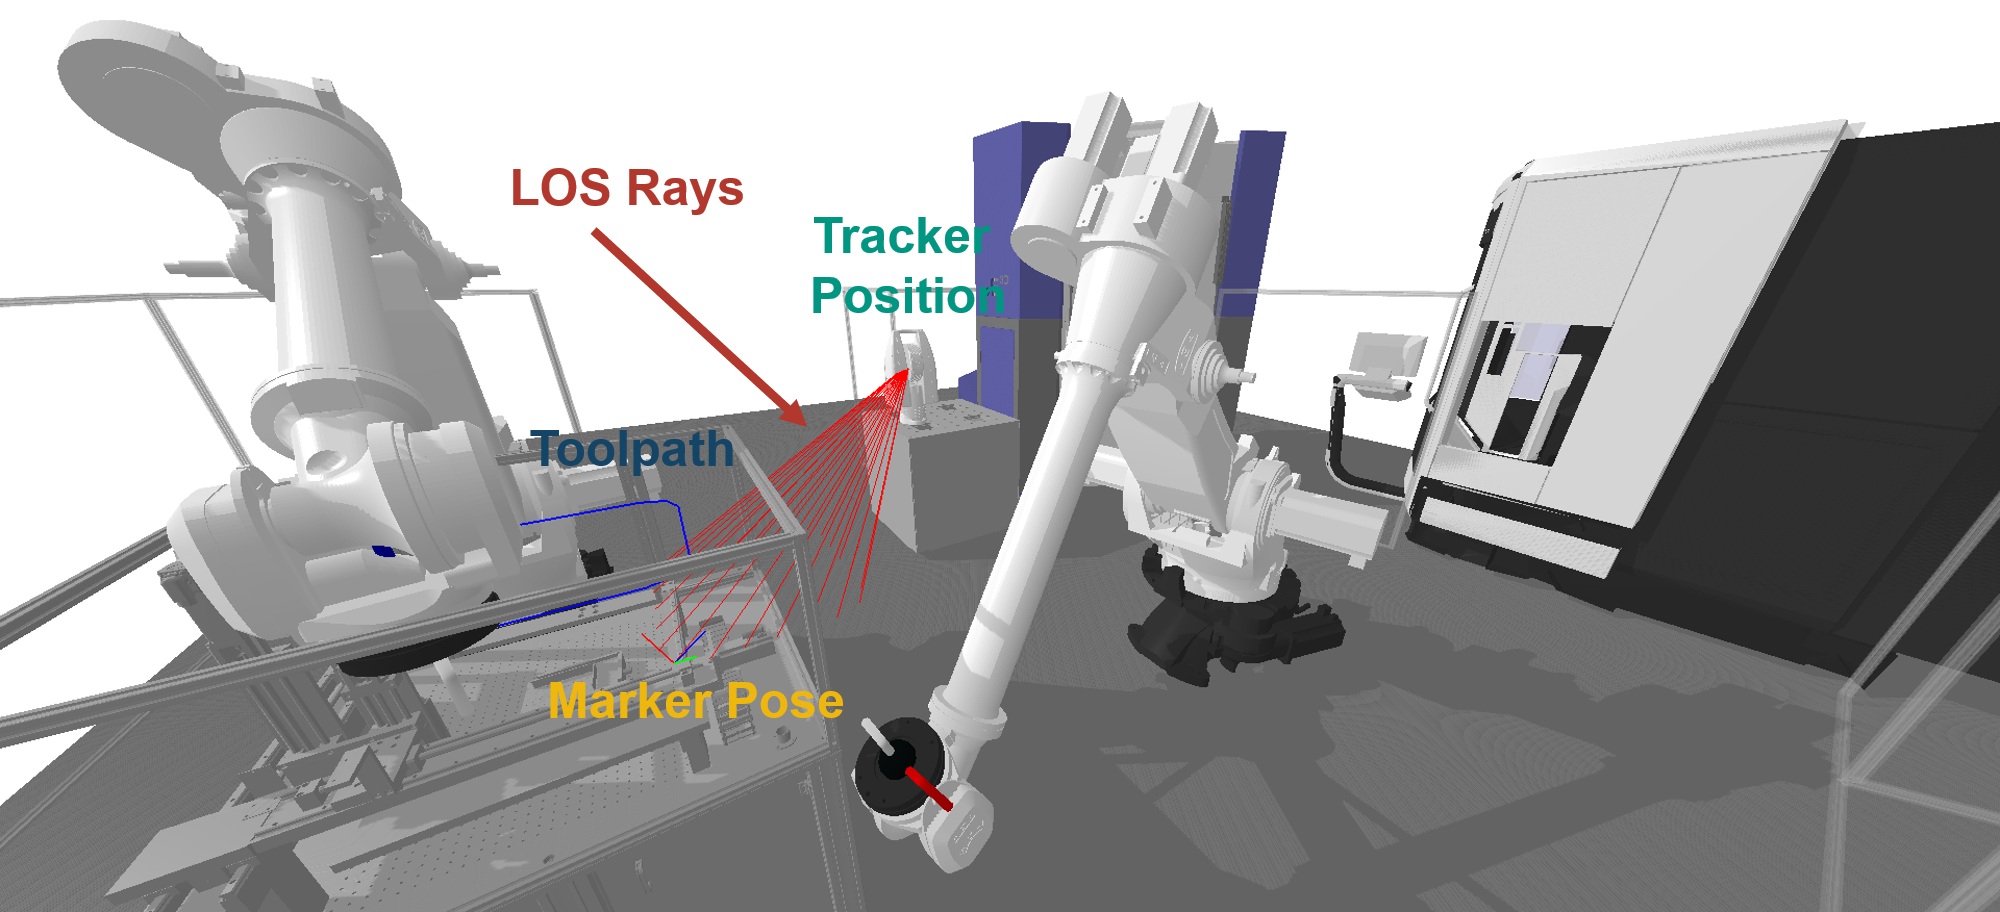
\includegraphics[width=0.9\textwidth]{figures/trajectory.png}
    \caption{Trajectory of the robot and final laser tracker and marker placements.}
    \label{fig:trajectory}
\end{figure}
\begin{figure}
    \centering
    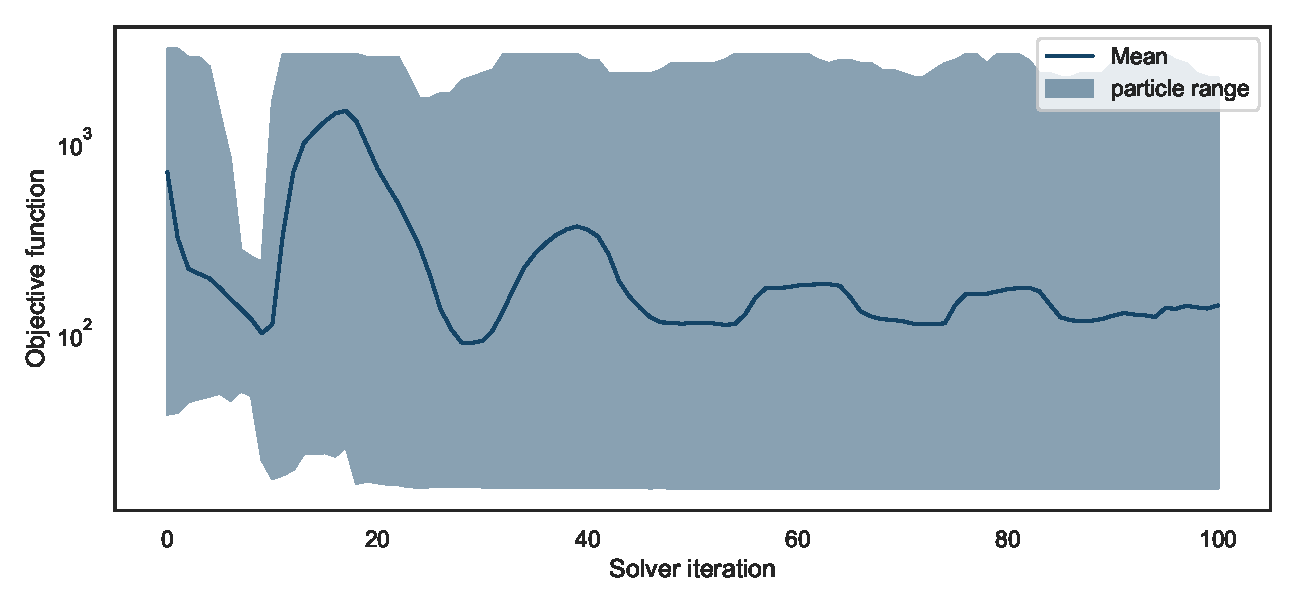
\includegraphics[width=0.9\textwidth]{figures/iterations.pdf}
    \caption{Performance of the algorithm over the iterations.}
    \label{fig:iterations}
\end{figure}

\section{Conclusion}
In this paper, we argue that automating the verification setup in manufacturing systems is feasible using optimization methods.
We demonstrated this with a particle swarm optimization algorithm that optimizes the placement of a laser tracker and markers.
Although initially labor-intensive, this approach proves beneficial for frequently reconfiguring systems as it requires only a simulation for each verification.
Our results confirm the algorithm's effectiveness in determining optimal sensor placements, significantly reducing the manual effort required by engineers.
We believe sensor placement optimization is a promising tool for researchers to verify system performance.
However, the field is nascent with several unanswered questions about integrating optimization in reconfiguration processes,
the potential for setup reuse across different designs, and developing multiple optimal solutions.
We hope this paper serves as a catalyst for further research in this domain.


\section{Acknowledgements}
This work was supported by the Ministry of Science, Research and Arts of the Federal State of Baden-Württemberg within the InnovationsCampus Future Mobility.
It was also funded by the Deutsche Forschungsgemeinschaft (DFG, German Research Foundation) - SFB-1574 - 471687386.
%Bibliography
%TODO checken ob das stimmt in template
\printbibliography

\end{document}

